\documentclass[a4paper,12pt]{scrartcl} %scrartcl
\usepackage[utf8]{inputenc}
%\usepackage{german}
\usepackage{amssymb}
\usepackage{amsmath}
% \usepackage{fancyhdr}
% \pagestyle{fancy}
\usepackage{tikz}
\usetikzlibrary{arrows,shapes,decorations.pathmorphing,backgrounds,patterns,positioning,fit,shadows,scopes}
\usepackage[margin=.7in]{geometry}

\newcommand{\tikzline}[2][3]{\raisebox{#1pt}{\tikz\draw (0,0)--(#2,0);}} %line with #1pts raise from (0,0) to (#2,0) [def of #2=15.2]

%sets left margins for itemize environments
\setlength\leftmargini{14pt}
\setlength\leftmarginii{12pt}
\setlength\leftmarginiii{14pt}


% \lhead{Nikolaus Mayer}
% \chead{SANDBOX}
% \rhead{\today}



\begin{document}

\begin{center}
  \begin{tikzpicture}[
      scale=1.5,%
      thin,%
      outerdouble/.style={double=white, double distance=1.75}%
    ]
    \draw (-.5,0)--(-5.5,0);
    \draw (.5,0)--(5.5,0);

    %\draw (0,0) circle (0.3);

    %% Diamond-hugging arcs
    \draw ({0-.05},-.3) arc (  0: 90:{.3-.05})
              ++(0, .1) arc (270:360:{.3-.05})
              ++(.1, 0) arc (180:270:{.3-.05})
              ++(0,-.1) arc ( 90:180:{.3-.05});

    %% Center diamond
    \draw[fill=black] (0,-.3) arc (  0: 90:.3) 
                              arc (270:360:.3)
                              arc (180:270:.3)
                              arc ( 90:180:.3) -- cycle;

    %\draw[outerdouble] ({0-.025},-.3) arc (  0: 90:{.3-.025});

    %% Surrounding white rectangle to clean up render artifacts
    %\draw[white,thick] (-.3,-.3)--++(.6,0)--++(0,.6)--++(-.6,0)--cycle;
          
    %\draw[fill=black] (0,-.3) arc (  0: 90:.3) 
    %                          arc (270:360:.3)
    %                          arc (180:270:.3)
    %                          arc ( 90:180:.3) -- cycle;
    %\draw (0,-.3) arc (0:90:.3) arc (270:0:.3);
  \end{tikzpicture}
\end{center}

$\;$\\\\
\begin{center}
  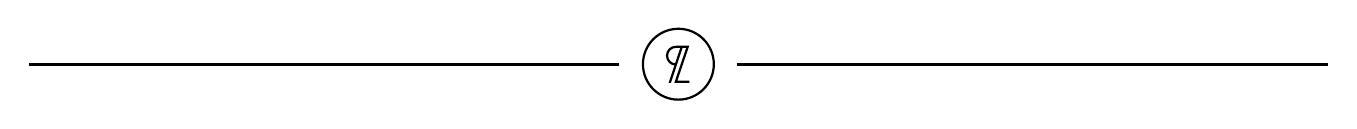
\begin{tikzpicture}[scale=1.5,thick]
    \draw[yshift=1.5] (0,0) circle (.3cm);

    {[xshift=-.6]
      %\draw (.1,-.095)--(0,-.095)--(.1,.2)--(0,.2);
      \draw (.115,-.095)--(0,-.095)--(.1,.2)--(0,.2);
      \draw (0,.2) arc (90:270:.075);
      \draw[shorten <= -.5pt] (-.05,-.1)--(.05,.2);
      \draw[white] (-.1,-.114)--++(.25,0);
    }

    \draw (-.5,.05)--(-5.5,.05);
    \draw (.5,.05)--(5.5,.05);
  \end{tikzpicture}
\end{center}

$\;$\\\\
\begin{center}
  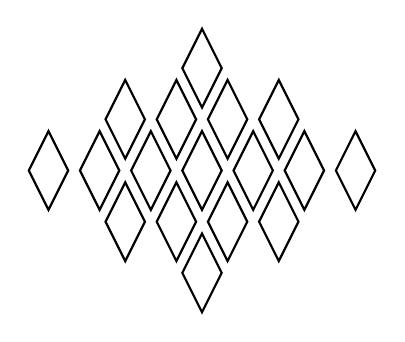
\begin{tikzpicture}[scale=.5,thick]
    \foreach \x/\y in {0/0, 1.3/0, .65/1.3, .65/-1.3, 1.95/-1.3, -.65/-1.3, 1.3/-2.6, 0/-2.6, .65/-3.9}
      \draw (-1+\x,0+\y)--(-1.5+\x,-1+\y)--(-2+\x,0+\y)--(-1.5+\x,1+\y)--cycle;
    \foreach \x/\y in {-1.95/-1.3, -1.3/0, -1.3/-2.6, -3.25/-1.3}
      \draw (-1+\x,0+\y)--(-1.5+\x,-1+\y)--(-2+\x,0+\y)--(-1.5+\x,1+\y)--cycle;
    \foreach \x/\y in {3.25/-1.3, 2.6/0, 2.6/-2.6, 4.55/-1.3}
      \draw (-1+\x,0+\y)--(-1.5+\x,-1+\y)--(-2+\x,0+\y)--(-1.5+\x,1+\y)--cycle;
  \end{tikzpicture}
\end{center}

$\;$\\\\
\begin{center}
  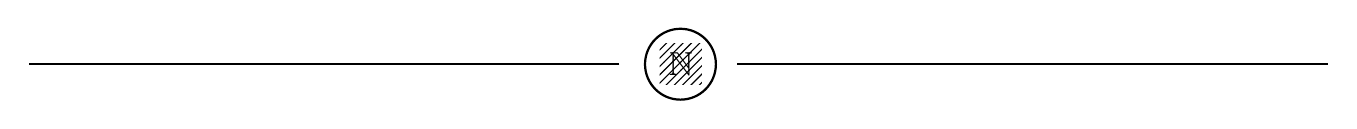
\begin{tikzpicture}[scale=1.5,thick]
    \draw[yshift=1.4,xshift=.5] (0,0) circle (.3cm);
    \node[pattern=north east lines] at (.02,.05) {\large $\mathbb{N}$};
    \draw (-.5,.05)--(-5.5,.05);
    \draw (.5,.05)--(5.5,.05);
  \end{tikzpicture}
\end{center}

$\;$\\\\
\begin{center}
  
\begin{tikzpicture}[scale=.5,thick]
    \foreach \x/\y in {0/0, 1.3/0, .65/1.3, .65/-1.3, 1.95/-1.3, -.65/-1.3, 1.3/-2.6, 0/-2.6, .65/-3.9}
      \draw[fill=blue,blue] (-1+\x,0+\y)--(-1.5+\x,-1+\y)--(-2+\x,0+\y)--(-1.5+\x,1+\y)--cycle;
    \foreach \x/\y in {-1.95/-1.3, -1.3/0, -1.3/-2.6, -3.25/-1.3}
      \draw [fill=blue!50,blue!50](-1+\x,0+\y)--(-1.5+\x,-1+\y)--(-2+\x,0+\y)--(-1.5+\x,1+\y)--cycle;
    \foreach \x/\y in {3.25/-1.3, 2.6/0, 2.6/-2.6}
      \draw[fill=blue!50,blue!50] (-1+\x,0+\y)--(-1.5+\x,-1+\y)--(-2+\x,0+\y)--(-1.5+\x,1+\y)--cycle;
    \foreach \x/\y in {-3.25/-1.3, 4.55/-1.3}
      \draw[fill=blue!30,blue!30] (-1+\x,0+\y)--(-1.5+\x,-1+\y)--(-2+\x,0+\y)--(-1.5+\x,1+\y)--cycle;
  \end{tikzpicture}
\end{center}

\pagebreak

\begin{center}
	\begin{tikzpicture}[scale=2]
		\foreach \x in {0,3,6}
			{
			\draw (\x,0)--++(60:1)--++(1,0)--++(-60:1)--++(1,0);
			\draw (\x,0)--++(-60:1)--++(1,0)--++(-60:1)--++(1,0) ++(-1,0)--++(240:1)--++(-1,0)--++(240:1);
			\draw (\x+2,0)--++(240:1) ++(-1,0)--++(240:1)--++(-60:1) ++(1,0)--++(-60:1)--++(1,0) ++(-1,0);
			\draw (\x+0.4,0) node{\ttfamily A-120};
			}

	\end{tikzpicture}
\end{center}


\pagebreak




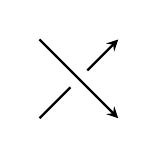
\begin{tikzpicture}
  \draw[->,thick,>=stealth] (0,0) -- (1,1);

  \draw[line width=3mm,>=stealth,white] (0,1) -- (1,0);
  \draw[->,thick,>=stealth] (0,1) -- (1,0);
\end{tikzpicture}



\tikzset{
  double arrow/.style args={#1 colored by #2 and #3}{
    -stealth,line width=#1,#2, % first arrow
    postaction={draw,-stealth,#3,line width=(#1)/3,
                shorten <=(#1)/3,shorten >=2*(#1)/3}, % second arrow
  }
}
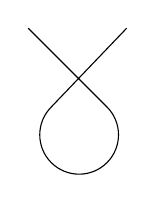
\begin{tikzpicture}
  \draw[double arrow=2mm colored by blue and white]
    (0,2) -- (1,1) arc(45:-360+45+90:.5) -- (1.25,2);
\end{tikzpicture}




\end{document}
